\section{Vectors basics}

Vectors are denoted by boldface letters such as $\mathbf{A}$. In Cartesian coordinates any vector in
3-dimensional space can be written as
\begin{equation}
    \mathbf{A} = A_x \mathbf{e}_x + A_y \mathbf{e}_y + A_z \mathbf{e}_z,
\end{equation}
and its magnitude is
\begin{equation}
    |\mathbf{A}| = \sqrt{A_x^2 + A_y^2 + A_z^2}.
\end{equation}

% The same ideas extend naturally from three dimensions to $\mathbb{R}^n$. An $n$-dimensional vector is an ordered list of components,
% \begin{equation}
%     \mathbf{v}=(v_1,v_2,\ldots,v_n)
%     =\sum_{i=1}^{n}v_i\mathbf{e}_i,
% \end{equation}
% where $\{\mathbf{e}_1,\ldots,\mathbf{e}_n\}$ is an orthonormal Cartesian basis. Two vectors are equal if and only if all corresponding components are equal.

% Vector addition and scalar multiplication are defined componentwise:
% \begin{equation}
%     \mathbf{u}+\mathbf{v}=(u_1+v_1,\ldots,u_n+v_n),
%     \qquad
%     a\mathbf{v}=(av_1,\ldots,av_n).
% \end{equation}
% The Euclidean inner product and norm are
% \begin{equation}
%     \mathbf{u}\cdot\mathbf{v}=\sum_{i=1}^{n}u_iv_i,
%     \qquad
%     \|\mathbf{v}\|=\sqrt{\mathbf{v}\cdot\mathbf{v}}
%     =\sqrt{\sum_{i=1}^{n}v_i^2}.
% \end{equation}
% The distance between two points represented by $\mathbf{u}$ and $\mathbf{v}$ is therefore
% \begin{equation}
%     d(\mathbf{u},\mathbf{v})=\|\mathbf{u}-\mathbf{v}\|
%     =\sqrt{\sum_{i=1}^{n}(u_i-v_i)^2}.
% \end{equation}

% The inner product determines the angle between two nonzero vectors:
% \begin{equation}
%     \cos\theta=\frac{\mathbf{u}\cdot\mathbf{v}}
%     {\|\mathbf{u}\|\,\|\mathbf{v}\|}.
% \end{equation}
% Thus $\mathbf{u}$ and $\mathbf{v}$ are orthogonal when $\mathbf{u}\cdot\mathbf{v}=0$. The Cauchy--Schwarz inequality,
% \begin{equation}
%     |\mathbf{u}\cdot\mathbf{v}|
%     \leq \|\mathbf{u}\|\,\|\mathbf{v}\|,
% \end{equation}
% ensures that this definition gives a real angle.

% The orthogonal projection of $\mathbf{v}$ onto a nonzero vector $\mathbf{u}$ is
% \begin{equation}
%     \operatorname{proj}_{\mathbf{u}}\mathbf{v}
%     =\frac{\mathbf{u}\cdot\mathbf{v}}{\mathbf{u}\cdot\mathbf{u}}\,\mathbf{u}.
% \end{equation}
% Consequently, every vector can be decomposed into components parallel and perpendicular to $\mathbf{u}$:
% \begin{equation}
%     \mathbf{v}=\operatorname{proj}_{\mathbf{u}}\mathbf{v}
%     +\left(\mathbf{v}-\operatorname{proj}_{\mathbf{u}}\mathbf{v}\right).
% \end{equation}

% For example, in $\mathbb{R}^4$ let
% \begin{equation}
%     \mathbf{u}=(1,2,0,-1),
%     \qquad
%     \mathbf{v}=(2,0,1,3).
% \end{equation}
% Then
% \begin{equation}
%     \mathbf{u}\cdot\mathbf{v}=1(2)+2(0)+0(1)+(-1)(3)=-1,
%     \qquad
%     \|\mathbf{u}\|^2=1^2+2^2+0^2+(-1)^2=6,
% \end{equation}
% so
% \begin{equation}
%     \operatorname{proj}_{\mathbf{u}}\mathbf{v}=-\frac{1}{6}\mathbf{u}
%     =\left(-\frac16,-\frac13,0,\frac16\right).
% \end{equation}

% The dot product and norm are defined in any dimension, whereas the familiar three-dimensional cross product $\mathbf{u}\times\mathbf{v}$ is a special operation in $\mathbb{R}^3$ (with a related two-dimensional scalar analogue). In general dimensions, antisymmetric products are represented using tensors such as the Levi-Civita symbol, as discussed in the index-notation section.


\subsection{Scalars and scaling}
A scalar is a quantity described only by magnitude (e.g. temperature, mass, charge). Multiplying a vector by a scalar scales its magnitude; a negative scalar reverses its direction:
\begin{equation}
    \alpha\mathbf{A}=\alpha A_x \mathbf{e}_x+\alpha A_y \mathbf{e}_y+\alpha A_z \mathbf{e}_z.
\end{equation}

\subsection{Addition and subtraction}
Vector addition and subtraction are performed componentwise:
\begin{equation}
    \mathbf{A}\pm\mathbf{B}=(A_x\pm B_x)\mathbf{e}_x+(A_y\pm B_y)\mathbf{e}_y+(A_z\pm B_z)\mathbf{e}_z.
\end{equation}
Geometrically, addition corresponds to the parallelogram rule; subtraction can be viewed by placing vectors head-to-tail so that $\mathbf{B}-\mathbf{A}$ is the vector from the tip of $\mathbf{A}$ to the tip of $\mathbf{B}$.

\begin{figure}[H]
    \centering
    
\includegraphics[width=0.6\textwidth]{figures/vec_sum_diff.png}
    \caption{Vector addition (parallelogram) and subtraction (head-to-tail).}
    \label{fig:vec_sum_diff}
\end{figure}

\begin{example}[Vector addition and subtraction]
Given
\begin{equation}
\mathbf{A}=4\mathbf{e}_x+4\mathbf{e}_y,
\qquad
\mathbf{B}=\mathbf{e}_x+8\mathbf{e}_y.
\end{equation}
Find the sum and difference and their magnitudes.

By componentwise addition,
\begin{equation}
\mathbf{S}=\mathbf{A}+\mathbf{B}=(4+1)\mathbf{e}_x+(4+8)\mathbf{e}_y=5\mathbf{e}_x+12\mathbf{e}_y,
\end{equation}
so
\begin{equation}
|\mathbf{S}|=\sqrt{5^2+12^2}=\sqrt{25+144}=\sqrt{169}=13.
\end{equation}
For the difference,
\begin{equation}
\mathbf{D}=\mathbf{B}-\mathbf{A}=(1-4)\mathbf{e}_x+(8-4)\mathbf{e}_y=-3\mathbf{e}_x+4\mathbf{e}_y,
\end{equation}
hence
\begin{equation}
|\mathbf{D}|=\sqrt{(-3)^2+4^2}=\sqrt{9+16}=\sqrt{25}=5.
\end{equation}
\end{example}

\subsection{Dot product}
The dot (scalar) product of two vectors is a scalar defined by
\begin{equation}
    \mathbf{A}\cdot\mathbf{B}=|\mathbf{A}|\,|\mathbf{B}|\cos\theta,
\end{equation}
where $\theta$ is the angle between them. In components,
\begin{equation}
    \mathbf{A}\cdot\mathbf{B}=A_xB_x+A_yB_y+A_zB_z.
\end{equation}

\begin{figure}[H]
    \centering
    
\includegraphics[width=0.5\textwidth]{figures/vec_dot_product.png}
    \caption{Dot product: projection and angle $\theta$.}
    \label{fig:vec_dot}
\end{figure}

\begin{example}[Angle from the dot product]
Given
\begin{equation}
\mathbf{A}=\sqrt{3}\,\mathbf{e}_x+\mathbf{e}_y,
\qquad
\mathbf{B}=2\mathbf{e}_x,
\end{equation}
find the angle $\theta$ between the two vectors.

First compute magnitudes:
\begin{equation}
|\mathbf{A}|=\sqrt{(\sqrt{3})^2+1^2}=2,
\qquad
|\mathbf{B}|=\sqrt{2^2}=2.
\end{equation}
Then compute the dot product:
\begin{equation}
\mathbf{A}\cdot\mathbf{B}=A_xB_x+A_yB_y=(\sqrt{3})(2)+1\cdot 0=2\sqrt{3}.
\end{equation}
Using $\mathbf{A}\cdot\mathbf{B}=|\mathbf{A}|\,|\mathbf{B}|\cos\theta$,
\begin{equation}
2\sqrt{3}=2\cdot 2\cos\theta=4\cos\theta,
\qquad
\cos\theta=\frac{\sqrt{3}}{2},
\end{equation}
thus
\begin{equation}
\theta=\cos^{-1}\!\left(\frac{\sqrt{3}}{2}\right)=30^\circ.
\end{equation}
\end{example}

\begin{example}[Water molecule bond angle]
Dot products are frequently used in molecular geometry. Let the oxygen atom be at the origin, and let
\begin{equation}
\mathrm{H}_1=(0.757,\,0,\,0.586),
\qquad
\mathrm{H}_2=(-0.757,\,0,\,0.586)
\end{equation}
in the $xz$-plane (units: \AA). Define bond vectors $\mathbf{u}=\overrightarrow{\mathrm{OH}_1}$ and $\mathbf{v}=\overrightarrow{\mathrm{OH}_2}$. Then
\begin{equation}
\cos\alpha=\frac{\mathbf{u}\cdot\mathbf{v}}{|\mathbf{u}|\,|\mathbf{v}|}
=\frac{0.586^2-0.757^2}{0.757^2+0.586^2}\approx -0.251,
\end{equation}
so
\begin{equation}
\alpha=\arccos(-0.251)\approx 104.5^\circ.
\end{equation}
Equivalently, if $\mathbf{u}=(a,0,b)$ and $\mathbf{v}=(-a,0,b)$, then
\begin{equation}
\cos\alpha=\frac{b^2-a^2}{a^2+b^2}.
\end{equation}
\end{example}

\begin{figure}[H]
    \centering
    
\includegraphics[width=0.5\textwidth]{figures/vec_water_bond_angle.png}
    \caption{Water molecule bond angle from a dot-product calculation.}
    \label{fig:water_bond}
\end{figure}

\begin{example}[Orthogonality test via dot product]
Given
\begin{equation}
\mathbf{p}=2\mathbf{e}_x-\mathbf{e}_y+2\mathbf{e}_z,
\qquad
\mathbf{q}=\mathbf{e}_x+2\mathbf{e}_y,
\end{equation}
determine whether $\mathbf{p}$ and $\mathbf{q}$ are perpendicular.

Compute the dot product:
\begin{equation}
\mathbf{p}\cdot\mathbf{q}=2\cdot 1+(-1)\cdot 2+2\cdot 0=2-2+0=0.
\end{equation}
Therefore, $\mathbf{p}\perp\mathbf{q}$.
\end{example}

\subsection{Cross product}
The cross (vector) product $\mathbf{A}\times\mathbf{B}$ is a vector perpendicular to both $\mathbf{A}$ and $\mathbf{B}$, with magnitude
\begin{equation}
    |\mathbf{A}\times\mathbf{B}|=|\mathbf{A}|\,|\mathbf{B}|\sin\theta,
\end{equation}
and direction given by the right-hand rule. Componentwise it may be written as the determinant
\begin{equation}
    \mathbf{A}\times\mathbf{B}=\begin{vmatrix}\mathbf{e}_x & \mathbf{e}_y & \mathbf{e}_z \\\\ A_x & A_y & A_z \\\\ B_x & B_y & B_z \end{vmatrix}.
\end{equation}

\begin{figure}[H]
    \centering
    
\includegraphics[width=0.5\textwidth]{figures/vec_cross_product.png}
    \caption{Cross product: right-hand rule and parallelogram area.}
    \label{fig:vec_cross}
\end{figure}

\begin{example}[Cross product and unit normal vector]
Given
\begin{equation}
\mathbf{A}=-\mathbf{e}_x+\mathbf{e}_y+\mathbf{e}_z,
\qquad
\mathbf{B}=\mathbf{e}_x-\mathbf{e}_y+\mathbf{e}_z,
\end{equation}
find a unit vector $\mathbf{e}_n$ perpendicular to both vectors (right-hand orientation), and find the angle between $\mathbf{A}$ and $\mathbf{B}$.

First compute
\begin{equation}
\mathbf{A}\times\mathbf{B}=\begin{vmatrix}
\mathbf{e}_x&\mathbf{e}_y&\mathbf{e}_z\\
-1&1&1\\
1&-1&1
\end{vmatrix}
=2\mathbf{e}_x+2\mathbf{e}_y.
\end{equation}
Its magnitude is
\begin{equation}
|\mathbf{A}\times\mathbf{B}|=\sqrt{2^2+2^2}=2\sqrt{2},
\end{equation}
so the unit normal is
\begin{equation}
\mathbf{e}_n=\frac{\mathbf{A}\times\mathbf{B}}{|\mathbf{A}\times\mathbf{B}|}
=\frac{1}{\sqrt{2}}\left(\mathbf{e}_x+\mathbf{e}_y\right).
\end{equation}

For the angle, compute
\begin{equation}
\mathbf{A}\cdot\mathbf{B}=(-1)(1)+1(-1)+1(1)=-1,
\end{equation}
and
\begin{equation}
|\mathbf{A}|=\sqrt{3},
\qquad
|\mathbf{B}|=\sqrt{3}.
\end{equation}
Hence
\begin{equation}
\cos\theta=\frac{\mathbf{A}\cdot\mathbf{B}}{|\mathbf{A}|\,|\mathbf{B}|}=-\frac{1}{3},
\qquad
\theta=\cos^{-1}\!\left(-\frac{1}{3}\right)\approx 109.47^\circ.
\end{equation}
\end{example}

\subsection{Scalar triple product}
The scalar triple product may be written equivalently as $(\mathbf{A}\times\mathbf{B})\cdot\mathbf{C}$ or $\mathbf{A}\cdot(\mathbf{B}\times\mathbf{C})$. Its magnitude equals the volume of the parallelepiped spanned by $\mathbf{A}$, $\mathbf{B}$, and $\mathbf{C}$; its sign records the orientation of the three vectors.

\begin{equation}
\mathbf{A}\cdot(\mathbf{B}\times\mathbf{C})
= A_x(B_yC_z-B_zC_y)+A_y(B_zC_x-B_xC_z)+A_z(B_xC_y-B_yC_x).
\end{equation}
Equivalently, it is the determinant
\begin{equation}
\mathbf{A}\cdot(\mathbf{B}\times\mathbf{C})
=\begin{vmatrix}
A_x & A_y & A_z \\
B_x & B_y & B_z \\
C_x & C_y & C_z
\end{vmatrix}.
\end{equation}
Interchanging the dot and cross products does not change the result:
\begin{equation}
\mathbf{A}\cdot(\mathbf{B}\times\mathbf{C})
=(\mathbf{A}\times\mathbf{B})\cdot\mathbf{C}.
\end{equation}
It is invariant under cyclic permutations and changes sign when any two vectors are exchanged. With
\begin{equation}
[\mathbf{A},\mathbf{B},\mathbf{C}]
=\mathbf{A}\cdot(\mathbf{B}\times\mathbf{C}),
\end{equation}
these properties are summarized by
\begin{equation}
\begin{aligned}
[\mathbf{A},\mathbf{B},\mathbf{C}]
&=[\mathbf{B},\mathbf{C},\mathbf{A}]
=[\mathbf{C},\mathbf{A},\mathbf{B}] \\
&=-[\mathbf{A},\mathbf{C},\mathbf{B}]
=-[\mathbf{B},\mathbf{A},\mathbf{C}]
=-[\mathbf{C},\mathbf{B},\mathbf{A}].
\end{aligned}
\end{equation}

\begin{figure}[H]
    \centering
    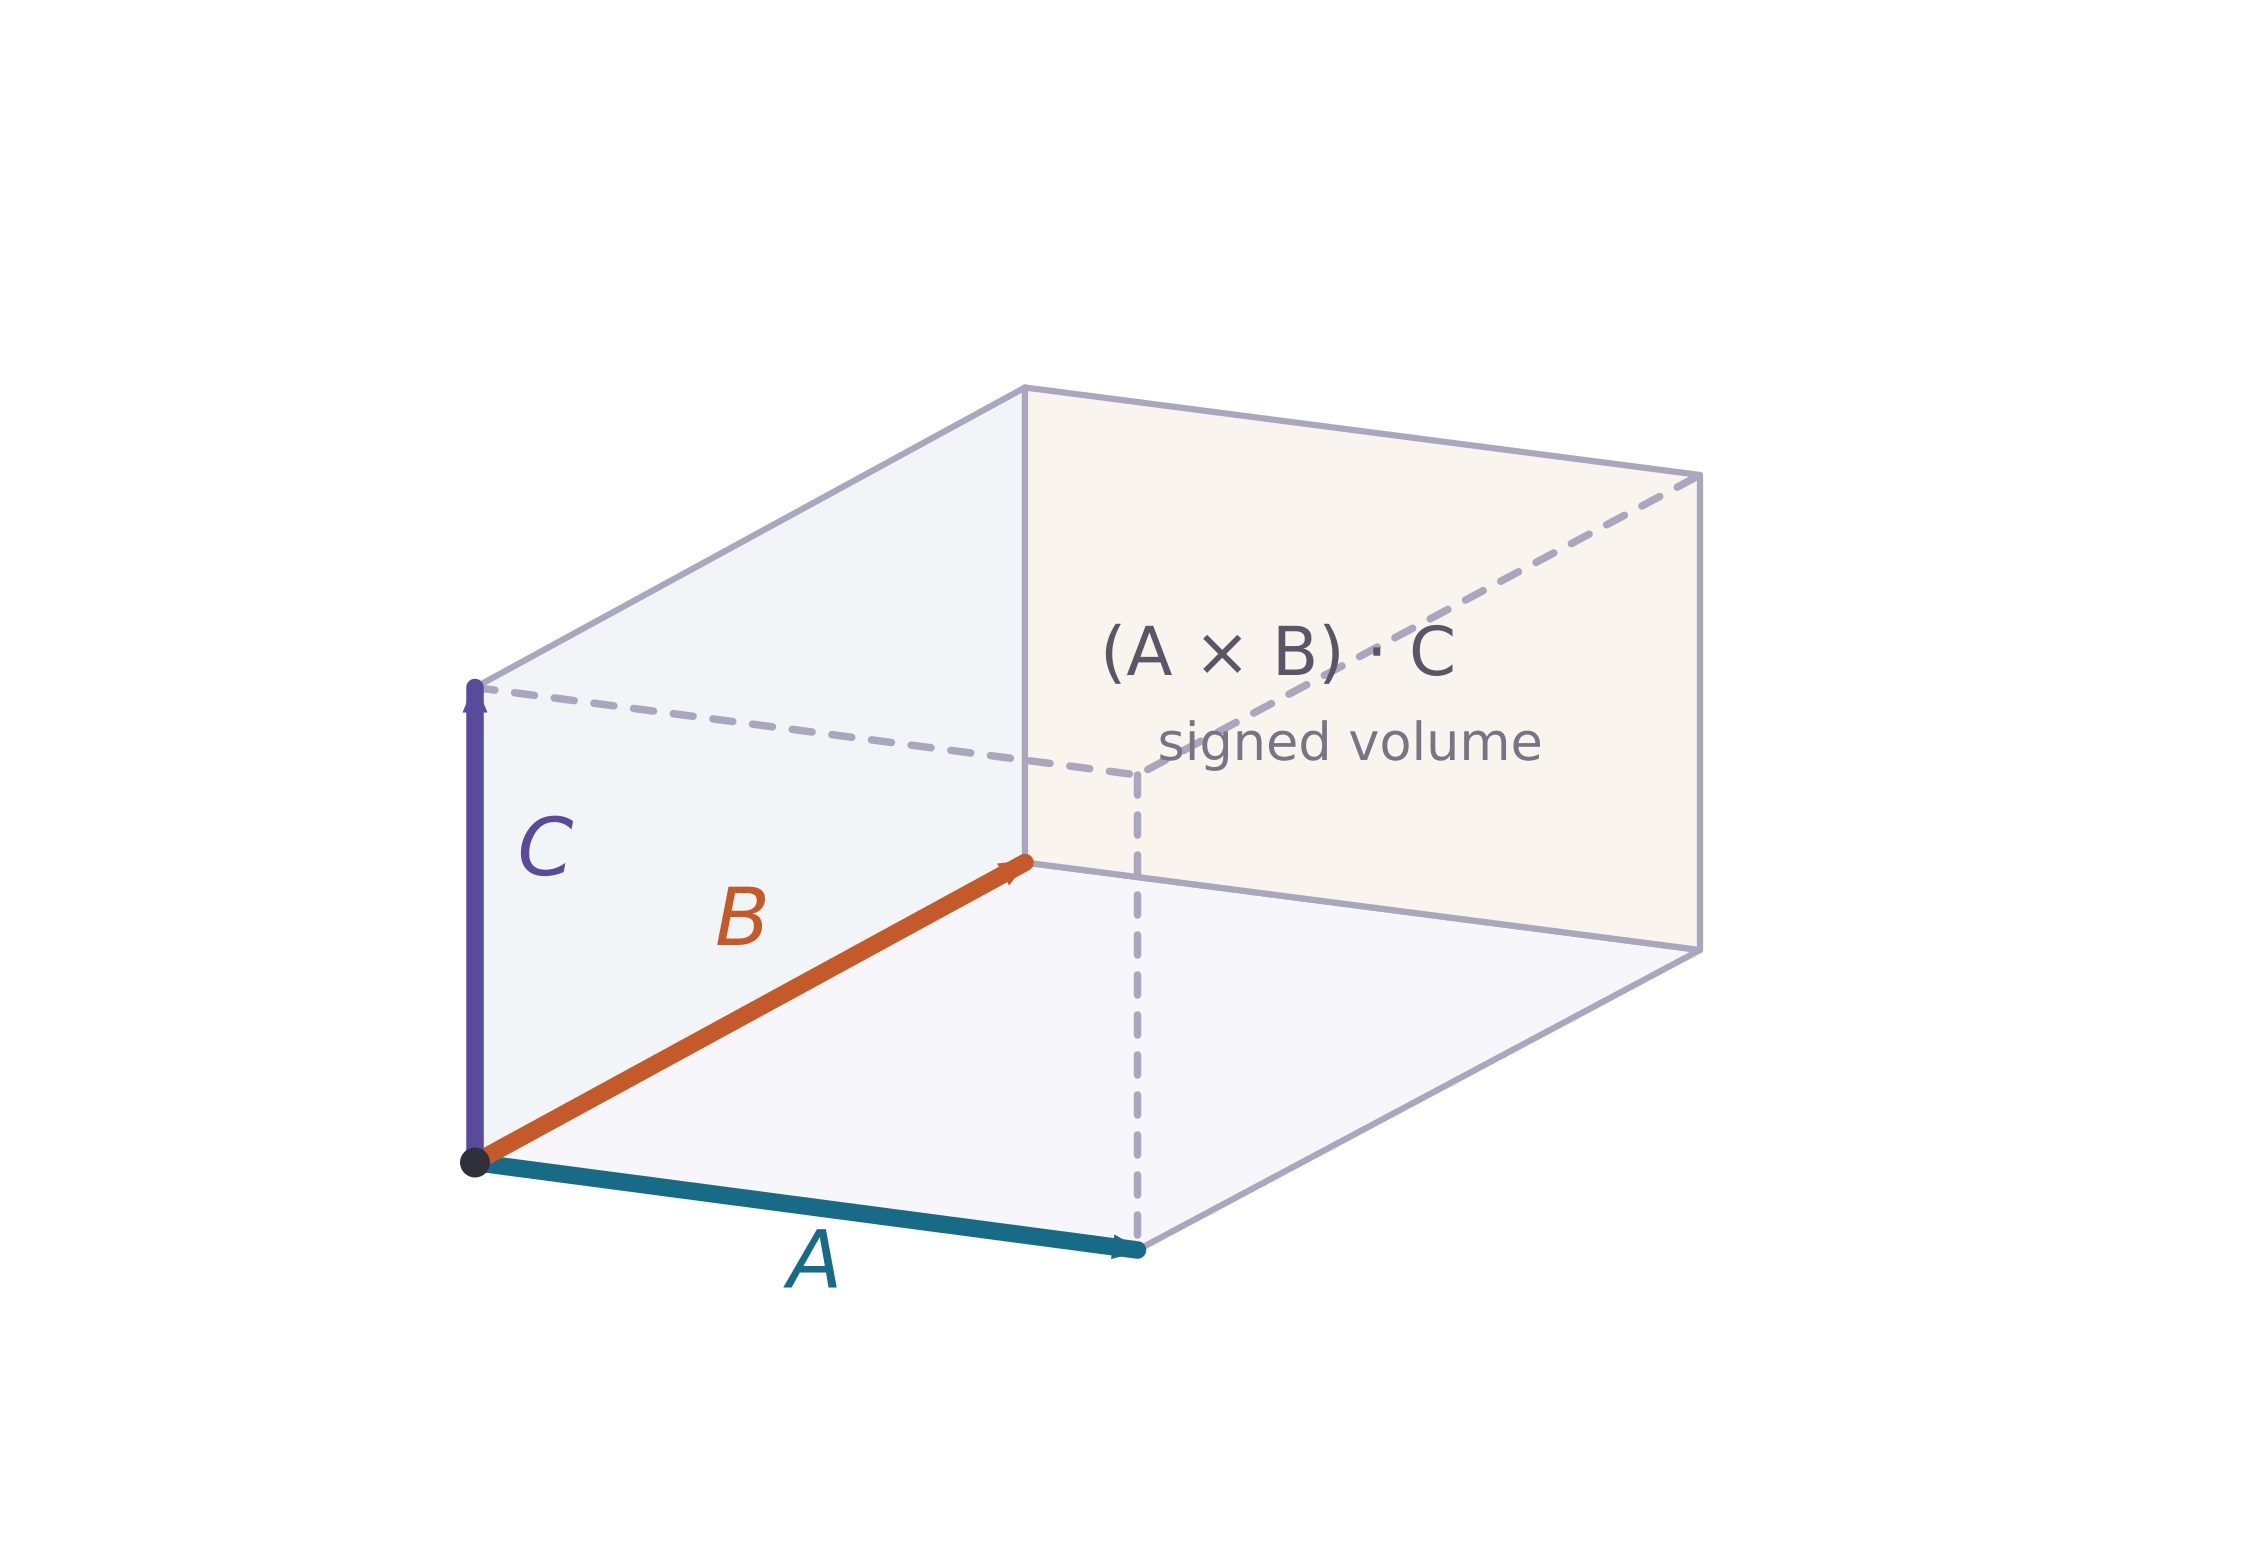
\includegraphics[width=0.5\textwidth]{figures/vec_scalar_triple_product.png}
    \caption{Scalar triple product as the signed volume of a parallelepiped.}
    \label{fig:scalar_triple_product}
\end{figure}

    Another useful identity involving both scalar and vector products is Lagrange's identity:
    \begin{equation}
    (\mathbf{A}\times\mathbf{B})\cdot(\mathbf{C}\times\mathbf{D})
    =(\mathbf{A}\cdot\mathbf{C})(\mathbf{B}\cdot\mathbf{D})
    -(\mathbf{A}\cdot\mathbf{D})(\mathbf{B}\cdot\mathbf{C}).
    \end{equation}

\begin{example}[Scalar triple product and volume]
Let
\begin{equation}
\mathbf{A}=\mathbf{e}_x+\mathbf{e}_y,
\qquad
\mathbf{B}=\mathbf{e}_y+\mathbf{e}_z,
\qquad
\mathbf{C}=\mathbf{e}_x+\mathbf{e}_z.
\end{equation}
Find $(\mathbf{A}\times\mathbf{B})\cdot\mathbf{C}$ and the corresponding volume.

First,
\begin{equation}
\mathbf{A}\times\mathbf{B}=
\begin{vmatrix}
\mathbf{e}_x & \mathbf{e}_y & \mathbf{e}_z \\
1 & 1 & 0 \\
0 & 1 & 1
\end{vmatrix}
=\mathbf{e}_x-\mathbf{e}_y+\mathbf{e}_z.
\end{equation}
Then
\begin{equation}
(\mathbf{A}\times\mathbf{B})\cdot\mathbf{C}
=(\mathbf{e}_x-\mathbf{e}_y+\mathbf{e}_z)\cdot(\mathbf{e}_x+\mathbf{e}_z)
=1+0+1=2.
\end{equation}
Hence the signed volume is $2$, and the geometric volume is $|2|=2$.
\end{example}

\subsection{Vector triple product}
The vector triple product of three vectors is a vector such as
$\mathbf{A}\times(\mathbf{B}\times\mathbf{C})$. It is perpendicular to
$\mathbf{A}$ and lies in the plane spanned by $\mathbf{B}$ and $\mathbf{C}$.
Unlike the scalar triple product, the cross product is not associative:
\begin{equation}
\mathbf{A}\times(\mathbf{B}\times\mathbf{C})
\ne(\mathbf{A}\times\mathbf{B})\times\mathbf{C}.
\end{equation}
The two useful reduction identities are
\begin{equation}
\mathbf{A}\times(\mathbf{B}\times\mathbf{C})
=(\mathbf{A}\cdot\mathbf{C})\mathbf{B}
-(\mathbf{A}\cdot\mathbf{B})\mathbf{C},
\end{equation}
and
\begin{equation}
(\mathbf{A}\times\mathbf{B})\times\mathbf{C}
=(\mathbf{A}\cdot\mathbf{C})\mathbf{B}
-(\mathbf{B}\cdot\mathbf{C})\mathbf{A}.
\end{equation}
They convert nested cross products into combinations of the original vectors.
For any three vectors, the cyclic sum also vanishes:
\begin{equation}
\mathbf{A}\times(\mathbf{B}\times\mathbf{C})
+\mathbf{B}\times(\mathbf{C}\times\mathbf{A})
+\mathbf{C}\times(\mathbf{A}\times\mathbf{B})=\mathbf{0}.
\end{equation}

\begin{example}[Projection perpendicular to a direction]
Let $\hat{\mathbf{n}}$ be a unit vector. Applying the first triple-product identity gives
\begin{equation}
\hat{\mathbf{n}}\times(\mathbf{v}\times\hat{\mathbf{n}})
=(\hat{\mathbf{n}}\cdot\hat{\mathbf{n}})\mathbf{v}
-(\hat{\mathbf{n}}\cdot\mathbf{v})\hat{\mathbf{n}}
=\mathbf{v}-(\mathbf{v}\cdot\hat{\mathbf{n}})\hat{\mathbf{n}}.
\end{equation}
Thus $\hat{\mathbf{n}}\times(\mathbf{v}\times\hat{\mathbf{n}})$ is precisely the component of $\mathbf{v}$ perpendicular to $\hat{\mathbf{n}}$.

For example, with $\mathbf{v}=2\mathbf{e}_x-\mathbf{e}_y+3\mathbf{e}_z$ and $\hat{\mathbf{n}}=\mathbf{e}_z$,
\begin{equation}
\hat{\mathbf{n}}\times(\mathbf{v}\times\hat{\mathbf{n}})
=\mathbf{v}-(\mathbf{v}\cdot\mathbf{e}_z)\mathbf{e}_z
=2\mathbf{e}_x-\mathbf{e}_y.
\end{equation}
This form is used to separate transverse and longitudinal components, for example when resolving motion or fields relative to a preferred direction.
\end{example}

% \begin{definition}
% A definition is a precise statement of meaning.
% \end{definition}


\subsection{From vectors to matrices}
Several vectors can be collected as the columns of a matrix. For example,
\begin{equation}
    M=\begin{pmatrix}\,|&|&|\\
    \mathbf{a}_1&\mathbf{a}_2&\mathbf{a}_3\\
    \,|&|&|
    \end{pmatrix}
    =\begin{pmatrix}
    a_{11}&a_{12}&a_{13}\\
    a_{21}&a_{22}&a_{23}\\
    a_{31}&a_{32}&a_{33}
    \end{pmatrix}.
\end{equation}
The matrix acts on a vector by taking a linear combination of its columns:
\begin{equation}
    M\mathbf{x}
    =x_1\mathbf{a}_1+x_2\mathbf{a}_2+x_3\mathbf{a}_3.
\end{equation}
Thus a matrix represents a linear transformation: it can rotate, stretch, reflect, or shear vectors. In components,
\begin{equation}
    (M\mathbf{x})_i=M_{ij}x_j,
\end{equation}
where the repeated index $j$ is summed. Applying two matrices in succession gives matrix multiplication,
\begin{equation}
    M(N\mathbf{x})=(MN)\mathbf{x}.
\end{equation}
The columns of the identity matrix are the basis vectors, so $I\mathbf{x}=\mathbf{x}$.
